% Options for packages loaded elsewhere
\PassOptionsToPackage{unicode}{hyperref}
\PassOptionsToPackage{hyphens}{url}
\PassOptionsToPackage{dvipsnames,svgnames*,x11names*}{xcolor}
%
\documentclass[
  10pt,
]{article}
\usepackage{lmodern}
\usepackage{setspace}
\usepackage{amssymb,amsmath}
\usepackage{ifxetex,ifluatex}
\ifnum 0\ifxetex 1\fi\ifluatex 1\fi=0 % if pdftex
  \usepackage[T1]{fontenc}
  \usepackage[utf8]{inputenc}
  \usepackage{textcomp} % provide euro and other symbols
\else % if luatex or xetex
  \usepackage{unicode-math}
  \defaultfontfeatures{Scale=MatchLowercase}
  \defaultfontfeatures[\rmfamily]{Ligatures=TeX,Scale=1}
  \setmainfont[]{DejaVu Serif}
  \setmonofont[]{DejaVu Sans Mono}
\fi
% Use upquote if available, for straight quotes in verbatim environments
\IfFileExists{upquote.sty}{\usepackage{upquote}}{}
\IfFileExists{microtype.sty}{% use microtype if available
  \usepackage[]{microtype}
  \UseMicrotypeSet[protrusion]{basicmath} % disable protrusion for tt fonts
}{}
\makeatletter
\@ifundefined{KOMAClassName}{% if non-KOMA class
  \IfFileExists{parskip.sty}{%
    \usepackage{parskip}
  }{% else
    \setlength{\parindent}{0pt}
    \setlength{\parskip}{6pt plus 2pt minus 1pt}}
}{% if KOMA class
  \KOMAoptions{parskip=half}}
\makeatother
\usepackage{xcolor}
\IfFileExists{xurl.sty}{\usepackage{xurl}}{} % add URL line breaks if available
\IfFileExists{bookmark.sty}{\usepackage{bookmark}}{\usepackage{hyperref}}
\hypersetup{
  colorlinks=true,
  linkcolor=red,
  filecolor=red,
  citecolor=red,
  urlcolor=red,
  pdfcreator={LaTeX via pandoc}}
\urlstyle{same} % disable monospaced font for URLs
\usepackage[margin=0.7cm,top=0.7cm,bottom=0.7cm,left=0.7cm,right=0.7cm,includeheadfoot]{geometry}
\usepackage{color}
\usepackage{fancyvrb}
\newcommand{\VerbBar}{|}
\newcommand{\VERB}{\Verb[commandchars=\\\{\}]}
\DefineVerbatimEnvironment{Highlighting}{Verbatim}{commandchars=\\\{\}}
% Add ',fontsize=\small' for more characters per line
\newenvironment{Shaded}{}{}
\newcommand{\AlertTok}[1]{\textcolor[rgb]{1.00,0.00,0.00}{\textbf{#1}}}
\newcommand{\AnnotationTok}[1]{\textcolor[rgb]{0.38,0.63,0.69}{\textbf{\textit{#1}}}}
\newcommand{\AttributeTok}[1]{\textcolor[rgb]{0.49,0.56,0.16}{#1}}
\newcommand{\BaseNTok}[1]{\textcolor[rgb]{0.25,0.63,0.44}{#1}}
\newcommand{\BuiltInTok}[1]{#1}
\newcommand{\CharTok}[1]{\textcolor[rgb]{0.25,0.44,0.63}{#1}}
\newcommand{\CommentTok}[1]{\textcolor[rgb]{0.38,0.63,0.69}{\textit{#1}}}
\newcommand{\CommentVarTok}[1]{\textcolor[rgb]{0.38,0.63,0.69}{\textbf{\textit{#1}}}}
\newcommand{\ConstantTok}[1]{\textcolor[rgb]{0.53,0.00,0.00}{#1}}
\newcommand{\ControlFlowTok}[1]{\textcolor[rgb]{0.00,0.44,0.13}{\textbf{#1}}}
\newcommand{\DataTypeTok}[1]{\textcolor[rgb]{0.56,0.13,0.00}{#1}}
\newcommand{\DecValTok}[1]{\textcolor[rgb]{0.25,0.63,0.44}{#1}}
\newcommand{\DocumentationTok}[1]{\textcolor[rgb]{0.73,0.13,0.13}{\textit{#1}}}
\newcommand{\ErrorTok}[1]{\textcolor[rgb]{1.00,0.00,0.00}{\textbf{#1}}}
\newcommand{\ExtensionTok}[1]{#1}
\newcommand{\FloatTok}[1]{\textcolor[rgb]{0.25,0.63,0.44}{#1}}
\newcommand{\FunctionTok}[1]{\textcolor[rgb]{0.02,0.16,0.49}{#1}}
\newcommand{\ImportTok}[1]{#1}
\newcommand{\InformationTok}[1]{\textcolor[rgb]{0.38,0.63,0.69}{\textbf{\textit{#1}}}}
\newcommand{\KeywordTok}[1]{\textcolor[rgb]{0.00,0.44,0.13}{\textbf{#1}}}
\newcommand{\NormalTok}[1]{#1}
\newcommand{\OperatorTok}[1]{\textcolor[rgb]{0.40,0.40,0.40}{#1}}
\newcommand{\OtherTok}[1]{\textcolor[rgb]{0.00,0.44,0.13}{#1}}
\newcommand{\PreprocessorTok}[1]{\textcolor[rgb]{0.74,0.48,0.00}{#1}}
\newcommand{\RegionMarkerTok}[1]{#1}
\newcommand{\SpecialCharTok}[1]{\textcolor[rgb]{0.25,0.44,0.63}{#1}}
\newcommand{\SpecialStringTok}[1]{\textcolor[rgb]{0.73,0.40,0.53}{#1}}
\newcommand{\StringTok}[1]{\textcolor[rgb]{0.25,0.44,0.63}{#1}}
\newcommand{\VariableTok}[1]{\textcolor[rgb]{0.10,0.09,0.49}{#1}}
\newcommand{\VerbatimStringTok}[1]{\textcolor[rgb]{0.25,0.44,0.63}{#1}}
\newcommand{\WarningTok}[1]{\textcolor[rgb]{0.38,0.63,0.69}{\textbf{\textit{#1}}}}
\usepackage{longtable,booktabs}
% Correct order of tables after \paragraph or \subparagraph
\usepackage{etoolbox}
\makeatletter
\patchcmd\longtable{\par}{\if@noskipsec\mbox{}\fi\par}{}{}
\makeatother
% Allow footnotes in longtable head/foot
\IfFileExists{footnotehyper.sty}{\usepackage{footnotehyper}}{\usepackage{footnote}}
\makesavenoteenv{longtable}
\setlength{\emergencystretch}{3em} % prevent overfull lines
\providecommand{\tightlist}{%
  \setlength{\itemsep}{0pt}\setlength{\parskip}{0pt}}
\setcounter{secnumdepth}{3}
% Enable graphics inclusion and ensure figure numbering works
\usepackage{graphicx}
\renewcommand{\figurename}{Figure}

% Configure fonts for Unicode support with fallbacks
\usepackage{newunicodechar}
\newunicodechar{⁴}{\textsuperscript{4}}
\newunicodechar{₄}{\textsubscript{4}}

% Configure hyperref colors consistently
\AtBeginDocument{
% Override pandoc's hidelinks setting with consistent options
\hypersetup{
    colorlinks=true,
    allcolors=red,
    linkcolor=red,
    urlcolor=red,
    citecolor=red,
    filecolor=red,
    menucolor=red,
    linktoc=all
}
}

\title{Quadray Analytical Details and Methods}
\author{Daniel Ari Friedman\\ ORCID: 0000-0001-6232-9096\\ Email: daniel@activeinference.institute}
\date{August 14, 2025}

\begin{document}
\maketitle

{
\hypersetup{linkcolor=red}
\setcounter{tocdepth}{3}
\tableofcontents
}
\setstretch{1.0}
\hypertarget{quadray-analytical-details-equations-and-methods}{%
\section{Quadray Analytical Details, Equations, and
Methods}\label{quadray-analytical-details-equations-and-methods}}

Here we review the coordinate conventions, conversions, and methods for
working with Quadray coordinates. We also review some exact tetravolume
formulas and how to compute them.

\hypertarget{coxeter.4d-euclidean-eux2074-symmetry-groups-and-polytopes}{%
\subsection{Coxeter.4D (Euclidean E⁴): symmetry groups and
polytopes}\label{coxeter.4d-euclidean-eux2074-symmetry-groups-and-polytopes}}

\begin{itemize}
\tightlist
\item
  \textbf{Setting}: standard Euclidean four-space E⁴ with orthogonal
  axes and Euclidean metric. This is the proper home for classical
  regular polytopes and their reflection symmetries. See background in
  Coxeter's Regular Polytopes (Dover), especially the clarification that
  Euclidean 4D is not spacetime (p.~119), and Conway \& Sloane's
  treatment of higher-dimensional lattices and packings.
\item
  \textbf{Coxeter groups}: generated by reflections with relations
  encoded by the Coxeter matrix \(m_{ij}\). The abstract group is
  defined by
\end{itemize}

\begin{equation}\label{eq:coxeter_relations}
(s_i s_j)^{m_{ij}} = e,\quad m_{ii}=1,\; m_{ij}\in\{2,3,4,\ldots,\infty\}\,.
\end{equation}

\begin{itemize}
\tightlist
\item
  \textbf{Gram matrix and angles}: for a Coxeter system realized by unit
  normal vectors to reflection hyperplanes, the Gram matrix is
\end{itemize}

\begin{equation}\label{eq:coxeter_gram}
G_{ij} = \begin{cases}
1, & i=j \\
-\cos\!\left(\dfrac{\pi}{m_{ij}}\right), & i\ne j
\end{cases}
\end{equation}

\begin{itemize}
\tightlist
\item
  \textbf{4D regular polytopes and diagrams}: canonical finite Coxeter
  diagrams in 4D include:

  \begin{itemize}
  \tightlist
  \item
    \([3,3,3]\): symmetry of the 5-cell (pentachoron), the 4D simplex.
  \item
    \([4,3,3]\): symmetry of the 8-cell/16-cell pair
    (tesseract--cross-polytope).
  \item
    \([3,4,3]\): symmetry of the unique self-dual 24-cell. These
    diagrams compactly encode generating reflections and dihedral angles
    between mirrors, guiding constructions and projections of 4D
    polytopes. See references:
    \href{https://en.wikipedia.org/wiki/Regular_polytope}{Regular
    polytopes (Coxeter)} and
    \href{https://en.wikipedia.org/wiki/Coxeter_group}{Coxeter group};
    lattice context:
    \href{https://link.springer.com/book/10.1007/978-1-4757-6568-7}{Sphere
    Packings, Lattices and Groups (Conway \& Sloane, Springer)}.
  \end{itemize}
\item
  \textbf{Bridge to our methods}: when we compute Euclidean volumes from
  edge lengths (e.g., Cayley--Menger; Eq. \eqref{eq:cayley_menger}), we
  are operating squarely in the Coxeter.4D/Euclidean paradigm,
  independent of Quadray unit conventions.
\end{itemize}

\hypertarget{einstein.4d-minkowski-spacetime-metric-and-field-equations}{%
\subsection{Einstein.4D (Minkowski spacetime): metric and field
equations}\label{einstein.4d-minkowski-spacetime-metric-and-field-equations}}

\begin{itemize}
\tightlist
\item
  \textbf{Metric}: an indefinite inner product space with line element
  (mostly-plus convention) given in Eq. \eqref{eq:einstein_line_element}
  of the 4D namespaces section. The metric tensor is \(g_{\mu\nu}\).
\item
  \textbf{Einstein field equations (EFE)}: curvature responds to
  stress--energy per
\end{itemize}

\begin{equation}\label{eq:efe}
G_{\mu \nu} + \Lambda\, g_{\mu \nu} = \kappa\, T_{\mu \nu},\qquad \kappa = \frac{8\pi G}{c^4}\,.
\end{equation}

\begin{itemize}
\tightlist
\item
  \textbf{Einstein tensor}: defined from the Ricci tensor \(R_{\mu\nu}\)
  and scalar curvature \(R\) by
\end{itemize}

\begin{equation}\label{eq:einstein_tensor}
G_{\mu \nu} = R_{\mu \nu} - \tfrac{1}{2}\,R\, g_{\mu \nu},\qquad R = g^{\mu\nu} R_{\mu\nu}\,.
\end{equation}

\begin{itemize}
\tightlist
\item
  \textbf{Scope note}: we use Einstein.4D primarily as a metric/geodesic
  analogy when discussing information geometry (e.g., Fisher metric and
  natural gradient). Physical constants \(G,c,\Lambda\) do not appear in
  Quadray lattice methods and should not be mixed with IVM unit
  conventions. References:
  \href{https://en.wikipedia.org/wiki/Einstein_field_equations}{Einstein
  field equations},
  \href{https://en.wikipedia.org/wiki/Minkowski_space}{Minkowski space},
  \href{https://en.wikipedia.org/wiki/Fisher_information}{Fisher
  information}.
\end{itemize}

\hypertarget{fuller.4d-coordinates-and-normalization}{%
\subsection{Fuller.4D Coordinates and
Normalization}\label{fuller.4d-coordinates-and-normalization}}

\begin{itemize}
\tightlist
\item
  Quadray vector q = (a,b,c,d), a,b,c,d ≥ 0, with at least one
  coordinate zero under normalization.
\item
  Projective normalization can add/subtract (k,k,k,k) without changing
  direction; choose k to enforce non-negativity and one zero minimum.
\item
  Isotropic Vector Matrix (IVM): integer quadrays describe CCP sphere
  centers; the 12 permutations of \{2,1,1,0\} form the cuboctahedron
  (vector equilibrium).

  \begin{itemize}
  \tightlist
  \item
    Integer-coordinate models: assigning unit IVM tetravolume to the
    regular tetrahedron yields integer coordinates for several familiar
    polyhedra (inverse tetrahedron, cube, octahedron, rhombic
    dodecahedron, cuboctahedron) when expressed as linear combinations
    of the four quadray basis vectors. See overview:
    \href{https://en.wikipedia.org/wiki/Quadray_coordinates}{Quadray
    coordinates}.
  \end{itemize}
\end{itemize}

\hypertarget{conversions-and-vector-operations-quadray-cartesian-fuller.4d-coxeter.4dxyz}{%
\subsection{Conversions and Vector Operations: Quadray ↔ Cartesian
(Fuller.4D ↔
Coxeter.4D/XYZ)}\label{conversions-and-vector-operations-quadray-cartesian-fuller.4d-coxeter.4dxyz}}

\begin{itemize}
\tightlist
\item
  \textbf{Embedding conventions} determine the linear maps between
  Quadray (Fuller.4D) and Cartesian XYZ (a 3D slice or embedding aligned
  with Coxeter.4D conventions).
\item
  \textbf{References}: Urner provides practical conversion write-ups and
  matrices; see:

  \begin{itemize}
  \tightlist
  \item
    Quadrays and XYZ:
    \href{https://www.grunch.net/synergetics/quadxyz.html}{Urner --
    Quadrays and XYZ}
  \item
    Introduction with examples:
    \href{https://www.grunch.net/synergetics/quadintro.html}{Urner --
    Quadray intro}
  \end{itemize}
\item
  \textbf{Implementation}: choose a fixed tetrahedral embedding;
  construct a 3×4 matrix M that maps (a,b,c,d) to (x,y,z), respecting
  A,B,C,D directions to tetra vertices. The inverse map can be defined
  up to projective normalization (adding (k,k,k,k)). When comparing
  volumes, use the \texttt{S3=\textbackslash{}sqrt\{9/8\}} scale to
  convert XYZ (Euclidean) volumes to IVM (Fuller.4D) units.
\item
  \textbf{Vector view}: treat \texttt{q} as a vector with magnitude and
  direction; define dot products and norms by pushing to XYZ via
  \texttt{M}.
\end{itemize}

\hypertarget{integer-coordinate-constructions-compact-derivation-box}{%
\subsubsection{Integer-coordinate constructions (compact derivation
box)}\label{integer-coordinate-constructions-compact-derivation-box}}

\begin{itemize}
\tightlist
\item
  Under the synergetics convention (unit regular tetrahedron has
  tetravolume 1), many familiar solids admit Quadray integer
  coordinates. For example, the octahedron at the same edge length has
  tetravolume 4, and its vertices can be formed as integer linear
  combinations of the four axes A,B,C,D subject to the Quadray
  normalization rule.
\item
  The cuboctahedron (vector equilibrium) arises as the shell of the 12
  nearest IVM neighbors given by the permutations of \((2,1,1,0)\). The
  rhombic dodecahedron (tetravolume 6) is the Voronoi cell of the
  FCC/CCP packing centered at the origin under the same embedding.
\item
  See Figure \ref{fig:polyhedra_quadray_map} for a schematic summary of
  these relationships.
\end{itemize}

\begin{longtable}[]{@{}lll@{}}
\toprule
\begin{minipage}[b]{0.30\columnwidth}\raggedright
Object\strut
\end{minipage} & \begin{minipage}[b]{0.30\columnwidth}\raggedright
Quadray construction (sketch)\strut
\end{minipage} & \begin{minipage}[b]{0.30\columnwidth}\raggedright
IVM volume\strut
\end{minipage}\tabularnewline
\midrule
\endhead
\begin{minipage}[t]{0.30\columnwidth}\raggedright
Regular tetrahedron\strut
\end{minipage} & \begin{minipage}[t]{0.30\columnwidth}\raggedright
Vertices \texttt{o=(0,0,0,0)}, \texttt{p=(2,1,0,1)},
\texttt{q=(2,1,1,0)}, \texttt{r=(2,0,1,1)}\strut
\end{minipage} & \begin{minipage}[t]{0.30\columnwidth}\raggedright
1\strut
\end{minipage}\tabularnewline
\begin{minipage}[t]{0.30\columnwidth}\raggedright
Cube (same edge)\strut
\end{minipage} & \begin{minipage}[t]{0.30\columnwidth}\raggedright
Union of 3 mutually orthogonal rhombic belts wrapped on the tetra frame;
edges tracked by XYZ embedding; compare Figure
\ref{fig:polyhedra_quadray_map}\strut
\end{minipage} & \begin{minipage}[t]{0.30\columnwidth}\raggedright
3\strut
\end{minipage}\tabularnewline
\begin{minipage}[t]{0.30\columnwidth}\raggedright
Octahedron (same edge)\strut
\end{minipage} & \begin{minipage}[t]{0.30\columnwidth}\raggedright
Convex hull of mid-edges of the tetra frame (pairwise axis sums
normalized)\strut
\end{minipage} & \begin{minipage}[t]{0.30\columnwidth}\raggedright
4\strut
\end{minipage}\tabularnewline
\begin{minipage}[t]{0.30\columnwidth}\raggedright
Rhombic dodecahedron\strut
\end{minipage} & \begin{minipage}[t]{0.30\columnwidth}\raggedright
Voronoi cell of FCC/CCP packing at origin (dual to cuboctahedron)\strut
\end{minipage} & \begin{minipage}[t]{0.30\columnwidth}\raggedright
6\strut
\end{minipage}\tabularnewline
\begin{minipage}[t]{0.30\columnwidth}\raggedright
Cuboctahedron (vector equilibrium)\strut
\end{minipage} & \begin{minipage}[t]{0.30\columnwidth}\raggedright
Shell of the 12 nearest IVM neighbors: permutations of
\texttt{(2,1,1,0)}\strut
\end{minipage} & \begin{minipage}[t]{0.30\columnwidth}\raggedright
20\strut
\end{minipage}\tabularnewline
\bottomrule
\end{longtable}

Small coordinate examples (subset):

\begin{itemize}
\tightlist
\item
  Cuboctahedron neighbors (representatives): \texttt{(2,1,1,0)},
  \texttt{(2,1,0,1)}, \texttt{(2,0,1,1)}, \texttt{(1,2,1,0)}; the full
  shell is all distinct permutations.
\item
  Tetrahedron:
  \texttt{{[}(0,0,0,0),\ (2,1,0,1),\ (2,1,1,0),\ (2,0,1,1){]}}.
\end{itemize}

Short scripts (reproducibility):

\begin{Shaded}
\begin{Highlighting}[]
\ExtensionTok{python3}\NormalTok{ quadmath/scripts/vector\_equilibrium\_panels.py}
\ExtensionTok{python3}\NormalTok{ quadmath/scripts/polyhedra\_quadray\_constructions.py}
\end{Highlighting}
\end{Shaded}

Programmatic check (neighbors, equal radii, adjacency):

\begin{Shaded}
\begin{Highlighting}[]
\ImportTok{import}\NormalTok{ numpy }\ImportTok{as}\NormalTok{ np}
\ImportTok{from}\NormalTok{ examples }\ImportTok{import}\NormalTok{ example\_cuboctahedron\_vertices\_xyz}

\NormalTok{xyz }\OperatorTok{=}\NormalTok{ np.array(example\_cuboctahedron\_vertices\_xyz())}
\NormalTok{r }\OperatorTok{=}\NormalTok{ np.linalg.norm(xyz[}\DecValTok{0}\NormalTok{])}
\ControlFlowTok{assert}\NormalTok{ np.allclose(np.linalg.norm(xyz, axis}\OperatorTok{=}\DecValTok{1}\NormalTok{), r)}

\CommentTok{\# Touching neighbors have separation 2r}
\NormalTok{touch }\OperatorTok{=}\NormalTok{ []}
\ControlFlowTok{for}\NormalTok{ i }\KeywordTok{in} \BuiltInTok{range}\NormalTok{(}\BuiltInTok{len}\NormalTok{(xyz)):}
    \ControlFlowTok{for}\NormalTok{ j }\KeywordTok{in} \BuiltInTok{range}\NormalTok{(i}\OperatorTok{+}\DecValTok{1}\NormalTok{, }\BuiltInTok{len}\NormalTok{(xyz)):}
\NormalTok{        d }\OperatorTok{=}\NormalTok{ np.linalg.norm(xyz[i] }\OperatorTok{{-}}\NormalTok{ xyz[j])}
        \ControlFlowTok{if} \BuiltInTok{abs}\NormalTok{(d }\OperatorTok{{-}} \DecValTok{2}\OperatorTok{*}\NormalTok{r) }\OperatorTok{/}\NormalTok{ (}\DecValTok{2}\OperatorTok{*}\NormalTok{r) }\OperatorTok{\textless{}} \FloatTok{0.05}\NormalTok{:}
\NormalTok{            touch.append((i, j))}
\ControlFlowTok{assert} \BuiltInTok{len}\NormalTok{(touch) }\OperatorTok{\textgreater{}} \DecValTok{0}
\end{Highlighting}
\end{Shaded}

\hypertarget{example-vertex-lists-and-volume-checks-illustrative}{%
\subsubsection{Example vertex lists and volume checks
(illustrative)}\label{example-vertex-lists-and-volume-checks-illustrative}}

The following snippets use canonical IVM neighbor points (permutations
of \((2,1,1,0)\)) to illustrate simple decompositions consistent with
synergetics volumes. Each tetra volume is computed via
\texttt{ace\_tetravolume\_5x5} and summed.

Octahedron (V = 4) as four unit IVM tetras around the origin:

\begin{Shaded}
\begin{Highlighting}[]
\ImportTok{from}\NormalTok{ quadray }\ImportTok{import}\NormalTok{ Quadray, ace\_tetravolume\_5x5}

\NormalTok{o }\OperatorTok{=}\NormalTok{ Quadray(}\DecValTok{0}\NormalTok{,}\DecValTok{0}\NormalTok{,}\DecValTok{0}\NormalTok{,}\DecValTok{0}\NormalTok{)}
\NormalTok{T }\OperatorTok{=}\NormalTok{ [}
\NormalTok{    (Quadray(}\DecValTok{2}\NormalTok{,}\DecValTok{1}\NormalTok{,}\DecValTok{0}\NormalTok{,}\DecValTok{1}\NormalTok{), Quadray(}\DecValTok{2}\NormalTok{,}\DecValTok{1}\NormalTok{,}\DecValTok{1}\NormalTok{,}\DecValTok{0}\NormalTok{), Quadray(}\DecValTok{2}\NormalTok{,}\DecValTok{0}\NormalTok{,}\DecValTok{1}\NormalTok{,}\DecValTok{1}\NormalTok{)),}
\NormalTok{    (Quadray(}\DecValTok{1}\NormalTok{,}\DecValTok{2}\NormalTok{,}\DecValTok{0}\NormalTok{,}\DecValTok{1}\NormalTok{), Quadray(}\DecValTok{1}\NormalTok{,}\DecValTok{2}\NormalTok{,}\DecValTok{1}\NormalTok{,}\DecValTok{0}\NormalTok{), Quadray(}\DecValTok{0}\NormalTok{,}\DecValTok{2}\NormalTok{,}\DecValTok{1}\NormalTok{,}\DecValTok{1}\NormalTok{)),}
\NormalTok{    (Quadray(}\DecValTok{1}\NormalTok{,}\DecValTok{1}\NormalTok{,}\DecValTok{2}\NormalTok{,}\DecValTok{0}\NormalTok{), Quadray(}\DecValTok{1}\NormalTok{,}\DecValTok{0}\NormalTok{,}\DecValTok{2}\NormalTok{,}\DecValTok{1}\NormalTok{), Quadray(}\DecValTok{0}\NormalTok{,}\DecValTok{1}\NormalTok{,}\DecValTok{2}\NormalTok{,}\DecValTok{1}\NormalTok{)),}
\NormalTok{    (Quadray(}\DecValTok{2}\NormalTok{,}\DecValTok{0}\NormalTok{,}\DecValTok{1}\NormalTok{,}\DecValTok{1}\NormalTok{), Quadray(}\DecValTok{1}\NormalTok{,}\DecValTok{2}\NormalTok{,}\DecValTok{0}\NormalTok{,}\DecValTok{1}\NormalTok{), Quadray(}\DecValTok{0}\NormalTok{,}\DecValTok{1}\NormalTok{,}\DecValTok{2}\NormalTok{,}\DecValTok{1}\NormalTok{)),  }\CommentTok{\# representative variant}
\NormalTok{]}
\NormalTok{V\_oct }\OperatorTok{=} \BuiltInTok{sum}\NormalTok{(ace\_tetravolume\_5x5(o, a, b, c) }\ControlFlowTok{for}\NormalTok{ (a,b,c) }\KeywordTok{in}\NormalTok{ T)}
\end{Highlighting}
\end{Shaded}

Cube (V = 3) as three unit IVM tetras (orthant-like around the origin):

\begin{Shaded}
\begin{Highlighting}[]
\ImportTok{from}\NormalTok{ quadray }\ImportTok{import}\NormalTok{ Quadray, ace\_tetravolume\_5x5}

\NormalTok{o }\OperatorTok{=}\NormalTok{ Quadray(}\DecValTok{0}\NormalTok{,}\DecValTok{0}\NormalTok{,}\DecValTok{0}\NormalTok{,}\DecValTok{0}\NormalTok{)}
\NormalTok{triples }\OperatorTok{=}\NormalTok{ [}
\NormalTok{    (Quadray(}\DecValTok{2}\NormalTok{,}\DecValTok{1}\NormalTok{,}\DecValTok{0}\NormalTok{,}\DecValTok{1}\NormalTok{), Quadray(}\DecValTok{2}\NormalTok{,}\DecValTok{1}\NormalTok{,}\DecValTok{1}\NormalTok{,}\DecValTok{0}\NormalTok{), Quadray(}\DecValTok{2}\NormalTok{,}\DecValTok{0}\NormalTok{,}\DecValTok{1}\NormalTok{,}\DecValTok{1}\NormalTok{)),}
\NormalTok{    (Quadray(}\DecValTok{1}\NormalTok{,}\DecValTok{2}\NormalTok{,}\DecValTok{0}\NormalTok{,}\DecValTok{1}\NormalTok{), Quadray(}\DecValTok{1}\NormalTok{,}\DecValTok{2}\NormalTok{,}\DecValTok{1}\NormalTok{,}\DecValTok{0}\NormalTok{), Quadray(}\DecValTok{0}\NormalTok{,}\DecValTok{2}\NormalTok{,}\DecValTok{1}\NormalTok{,}\DecValTok{1}\NormalTok{)),}
\NormalTok{    (Quadray(}\DecValTok{1}\NormalTok{,}\DecValTok{1}\NormalTok{,}\DecValTok{2}\NormalTok{,}\DecValTok{0}\NormalTok{), Quadray(}\DecValTok{1}\NormalTok{,}\DecValTok{0}\NormalTok{,}\DecValTok{2}\NormalTok{,}\DecValTok{1}\NormalTok{), Quadray(}\DecValTok{0}\NormalTok{,}\DecValTok{1}\NormalTok{,}\DecValTok{2}\NormalTok{,}\DecValTok{1}\NormalTok{)),}
\NormalTok{]}
\NormalTok{V\_cube }\OperatorTok{=} \BuiltInTok{sum}\NormalTok{(ace\_tetravolume\_5x5(o, a, b, c) }\ControlFlowTok{for}\NormalTok{ (a,b,c) }\KeywordTok{in}\NormalTok{ triples)}
\end{Highlighting}
\end{Shaded}

Notes.

\begin{itemize}
\tightlist
\item
  These decompositions are illustrative and use canonical IVM neighbor
  triples that produce unit tetras under \texttt{ace\_tetravolume\_5x5}.
  Other equivalent tilings are possible.
\item
  Volumes are invariant to adding \((k,k,k,k)\) to each vertex of a
  tetra (projective normalization), which the 5×5 determinant respects.
\end{itemize}

\hypertarget{sec:integer_volume}{%
\subsection{Integer Volume Quantization}\label{sec:integer_volume}}

For a tetrahedron with vertices P₀..P₃ in the Quadray integer lattice
(Fuller.4D):

\begin{equation}\label{eq:lattice_det}
V = \tfrac{1}{6}\,\left|\det\,[\,P_1 - P_0,\; P_2 - P_0,\; P_3 - P_0\,]\right|
\end{equation}

\begin{itemize}
\tightlist
\item
  With integer coordinates, the determinant is integer; lattice
  tetrahedra yield integer volumes.
\item
  Unit conventions: regular tetrahedron volume = 1 (synergetics).
\end{itemize}

Notes.

\begin{itemize}
\tightlist
\item
  \(P_0,\ldots,P_3\) are tetrahedron vertices in Quadray coordinates.
\item
  \(V\) is the Euclidean volume measured in IVM tetra-units; the \(1/6\)
  factor converts the parallelepiped determinant to a tetra volume.
\item
  Background and variations are discussed under Tetrahedron volume
  formulas:
  \href{https://en.wikipedia.org/wiki/Tetrahedron\#Volume}{Tetrahedron
  -- volume}.
\end{itemize}

Tom Ace 5×5 determinant (tetravolume directly from quadrays):

\begin{equation}\label{eq:ace5x5}
V_{ivm} = \tfrac{1}{4} \left| \det \begin{pmatrix}
 a_0 & a_1 & a_2 & a_3 & 1 \\
 b_0 & b_1 & b_2 & b_3 & 1 \\
 c_0 & c_1 & c_2 & c_3 & 1 \\
 d_0 & d_1 & d_2 & d_3 & 1 \\
 1 & 1 & 1 & 1 & 0
\end{pmatrix} \right|
\end{equation}

This returns the same integer volumes for lattice tetrahedra. See the
implementation \texttt{ace\_tetravolume\_5x5}.

Notes.

\begin{itemize}
\tightlist
\item
  Rows correspond to the Quadray 4-tuples of the four vertices with a
  final affine column of ones; the last row enforces projective
  normalization.
\item
  The factor \(\tfrac{1}{4}\) returns tetravolumes in IVM units
  consistent with synergetics. See also
  \href{https://en.wikipedia.org/wiki/Quadray_coordinates}{Quadray
  coordinates}.
\end{itemize}

Equivalently, define the 5×5 matrix of quadray coordinates augmented
with an affine 1 as

\begin{equation}\label{eq:ace5x5_expanded}
M(q_0,q_1,q_2,q_3) = \begin{bmatrix}
q_{01} & q_{02} & q_{03} & q_{04} & 1 \\
q_{11} & q_{12} & q_{13} & q_{14} & 1 \\
q_{21} & q_{22} & q_{23} & q_{24} & 1 \\
q_{31} & q_{32} & q_{33} & q_{34} & 1 \\
1 & 1 & 1 & 1 & 0
\end{bmatrix},\qquad V_{ivm} = \tfrac{1}{4}\,\big|\det M(q_0,q_1,q_2,q_3)\big|\,.
\end{equation}

Points vs vectors: subtracting points is shorthand for forming edge
vectors. We treat quadray 4-tuples as vectors from the origin;
differences like \((P_1-P_0)\) mean ``edge vectors,'' avoiding ambiguity
between ``points'' and ``vectors.''

Equivalently via Cayley--Menger determinant (Coxeter.4D/Euclidean
lengths)
(\href{https://en.wikipedia.org/wiki/Cayley\%E2\%80\%93Menger_determinant}{Cayley--Menger
determinant}):

\begin{equation}\label{eq:cayley_menger}
288\,V^2 = \det\begin{pmatrix}
  0 & 1 & 1 & 1 & 1 \\
  1 & 0 & d_{01}^2 & d_{02}^2 & d_{03}^2 \\
  1 & d_{10}^2 & 0 & d_{12}^2 & d_{13}^2 \\
  1 & d_{20}^2 & d_{21}^2 & 0 & d_{23}^2 \\
  1 & d_{30}^2 & d_{31}^2 & d_{32}^2 & 0
\end{pmatrix}
\end{equation}

References:
\href{https://en.wikipedia.org/wiki/Cayley\%E2\%80\%93Menger_determinant}{Cayley--Menger
determinant}, lattice tetrahedra discussions in geometry texts; see also
\href{https://en.wikipedia.org/wiki/Tetrahedron\#Volume}{Tetrahedron --
volume}. Code: \texttt{integer\_tetra\_volume},
\texttt{ace\_tetravolume\_5x5}.

Notes.

\begin{itemize}
\tightlist
\item
  \textbf{Pairwise distances}: \(d_{ij}\) are Euclidean distances
  between vertices \(P_i\) and \(P_j\).
\item
  \textbf{Length-only formulation}: Cayley--Menger provides a
  length-only formula for simplex volumes, here specialized to
  tetrahedra; see the canonical reference above.
\end{itemize}

\begin{longtable}[]{@{}ll@{}}
\caption{Polyhedra tetravolumes in IVM units (edge length equal to the
unit tetra edge). \{\#tbl:polyhedra\_volumes\}}\tabularnewline
\toprule
Polyhedron (edge = tetra edge) & Volume (tetra-units)\tabularnewline
\midrule
\endfirsthead
\toprule
Polyhedron (edge = tetra edge) & Volume (tetra-units)\tabularnewline
\midrule
\endhead
Regular Tetrahedron & 1\tabularnewline
Cube & 3\tabularnewline
Octahedron & 4\tabularnewline
Rhombic Dodecahedron & 6\tabularnewline
Cuboctahedron (Vector Equilibrium) & 20\tabularnewline
\bottomrule
\end{longtable}

\hypertarget{distances-and-metrics}{%
\subsection{Distances and Metrics}\label{distances-and-metrics}}

Distance definitions depend on the chosen embedding and normalization.
For cross-references to information geometry, see
\href{08_equations_appendix.md\#eq:fim}{Eq. (FIM)} and
\href{08_equations_appendix.md\#eq:natgrad}{natural gradient} in the
Equations appendix.

\hypertarget{sec:xyz_conversion}{%
\subsection{XYZ determinant and S3
conversion}\label{sec:xyz_conversion}}

Given XYZ coordinates of tetrahedron vertices (x\_i, y\_i, z\_i), the
Euclidean volume is

\begin{equation}\label{eq:xyz_det}
V_{xyz} = \tfrac{1}{6} \left| \det \begin{pmatrix}
 x_a & y_a & z_a & 1 \\
 x_b & y_b & z_b & 1 \\
 x_c & y_c & z_c & 1 \\
 x_d & y_d & z_d & 1
\end{pmatrix} \right|
\end{equation}

Synergetics relates IVM and XYZ unit conventions via
\(S3 = \sqrt{9/8}\). Multiplying an XYZ volume by \(S3\) converts to IVM
tetra-units when the embedding uses \(R\)-edge unit cubes and \(D=2R\)
for quadray edges; see
\href{https://en.wikipedia.org/wiki/Synergetics_(Fuller)}{Synergetics
(Fuller)}.

Notes.

\begin{itemize}
\item
  \((x_\cdot,y_\cdot,z_\cdot)\) denote Cartesian coordinates of the four
  vertices; the affine column of ones yields a homogeneous-coordinate
  determinant for tetra volume.
\item
  Conversion to IVM units uses the synergetics scale \(S3=\sqrt{9/8}\).
\item
  Euclidean embedding distance via appropriate linear map from quadray
  to R³.
\item
  Information geometry metric: Fisher Information Matrix (FIM)

  \begin{itemize}
  \tightlist
  \item
    \(\mathrm{FIM}[i,j] = \mathbb{E}\big[\, \partial_{\theta_i} \log p(x;\theta)\,\partial_{\theta_j} \log p(x;\theta)\,\big]\)
  \item
    Acts as Riemannian metric; natural gradient uses FIM⁻¹ ∇θ L. See
    \href{https://en.wikipedia.org/wiki/Fisher_information}{Fisher
    information}.
  \end{itemize}
\end{itemize}

\hypertarget{fisher-geometry-in-quadray-space}{%
\subsection{Fisher Geometry in Quadray
Space}\label{fisher-geometry-in-quadray-space}}

\begin{itemize}
\tightlist
\item
  Symmetries of quadray lattices often induce near block-diagonal FIM.
\item
  Determinant and spectrum characterize conditioning and information
  concentration.
\end{itemize}

\hypertarget{practical-methods}{%
\subsection{Practical Methods}\label{practical-methods}}

\hypertarget{sec:tetravolumes_quadrays}{%
\subsection{Tetravolumes with
Quadrays}\label{sec:tetravolumes_quadrays}}

\begin{itemize}
\item
  The tetravolume of a tetrahedron with vertices given as Quadrays
  \texttt{a,b,c,d} can be computed directly from their 4-tuples via the
  Tom Ace 5×5 determinant; see Eq. \eqref{eq:ace5x5} for the canonical
  form.
\item
  Unit regular tetrahedron from origin: with \texttt{o=(0,0,0,0)},
  \texttt{p=(2,1,0,1)}, \texttt{q=(2,1,1,0)}, \texttt{r=(2,0,1,1)}, we
  have \texttt{V\_ivm(o,p,q,r)=1}. Doubling each vector scales volume by
  8, as expected.
\item
  Equivalent length-based formulas agree with the 5×5 determinant:

  \begin{itemize}
  \tightlist
  \item
    Cayley--Menger:
    \(288\,V^2 = \det\begin{pmatrix}0&1&1&1&1\\1&0&d_{01}^2&d_{02}^2&d_{03}^2\\1&d_{10}^2&0&d_{12}^2&d_{13}^2\\1&d_{20}^2&d_{21}^2&0&d_{23}^2\\1&d_{30}^2&d_{31}^2&d_{32}^2&0\end{pmatrix}\).
  \item
    Piero della Francesca (PdF) Heron-like formula (converted to IVM via
    \(S3 = \sqrt{9/8}\)).
  \end{itemize}

  Let edge lengths meeting at a vertex be \(a,b,c\), and the opposite
  edges be \(d,e,f\). The Euclidean volume satisfies

  \begin{equation}\label{eq:pdf}
  144\,V_{xyz}^2 = 4 a^2 b^2 c^2 - a^2\,(b^2 + c^2 - f^2)^2 - b^2\,(c^2 + a^2 - e^2)^2 - c^2\,(a^2 + b^2 - d^2)^2 + (b^2 + c^2 - f^2)(c^2 + a^2 - e^2)(a^2 + b^2 - d^2)\,.
  \end{equation}

  Convert to IVM units via \(V_{ivm} = S3 \cdot V_{xyz}\) with
  \(S3=\sqrt{9/8}\). See background discussion under
  \href{https://en.wikipedia.org/wiki/Tetrahedron\#Volume}{Tetrahedron
  -- volume}.
\item
  Gerald de Jong (GdJ) formula, which natively returns tetravolumes.

  In Quadray coordinates, one convenient native form uses edge-vector
  differences and an integer-preserving determinant (agreeing with Ace
  5×5):

  \begin{equation}\label{eq:gdj}
  V_{ivm} = \frac{1}{4}\,\left|\det \begin{pmatrix}
  a_1-a_0 & a_2-a_0 & a_3-a_0 \\
  b_1-b_0 & b_2-b_0 & b_3-b_0 \\
  c_1-c_0 & c_2-c_0 & c_3-c_0 \\
  \end{pmatrix}\right|\,.
  \end{equation}

  where each column is formed from Quadray component differences of
  \(P_1-P_0\), \(P_2-P_0\), \(P_3-P_0\) projected to a 3D slice
  consistent with the synergetics convention; integer arithmetic is
  exact and the factor \(\tfrac{1}{4}\) produces IVM tetravolumes. See
  de Jong's Quadray notes and Urner's implementations for derivations
  (\href{https://en.wikipedia.org/wiki/Quadray_coordinates}{Quadray
  coordinates}).
\end{itemize}

\hypertarget{bridging-vs-native-tetravolume-formulas-results-reference}{%
\subsubsection{Bridging vs native tetravolume formulas (Results
reference)}\label{bridging-vs-native-tetravolume-formulas-results-reference}}

\begin{itemize}
\tightlist
\item
  \textbf{Lengths (bridging)}: PdF and Cayley--Menger (CM) consume
  Cartesian lengths (XYZ) and produce Euclidean volumes; convert to IVM
  units via \(S3 = \sqrt{9/8}\).
\item
  \textbf{Quadray-native}: Gerald de Jong (GdJ) returns IVM tetravolumes
  directly (no XYZ bridge). Tom Ace's 5×5 coordinate formula is likewise
  native IVM. All agree numerically with CM+S3 on shared cases.
\end{itemize}

References and discussion:
\href{https://github.com/4dsolutions/School_of_Tomorrow/blob/master/tetravolume.py}{Urner
-- tetravolume.py (School of Tomorrow)},
\href{https://github.com/4dsolutions/School_of_Tomorrow/blob/master/VolumeTalk.ipynb}{Urner
-- VolumeTalk.ipynb}, \href{https://flic.kr/p/2rn22en}{Urner -- Flickr
diagram}.

Figure: automated comparison (native Ace 5×5 vs CM+S3) across small
examples (see script \texttt{sympy\_formalisms.py}). The figure and
source CSV/NPZ are in \texttt{quadmath/output/}.

\begin{figure}[htbp]
\centering
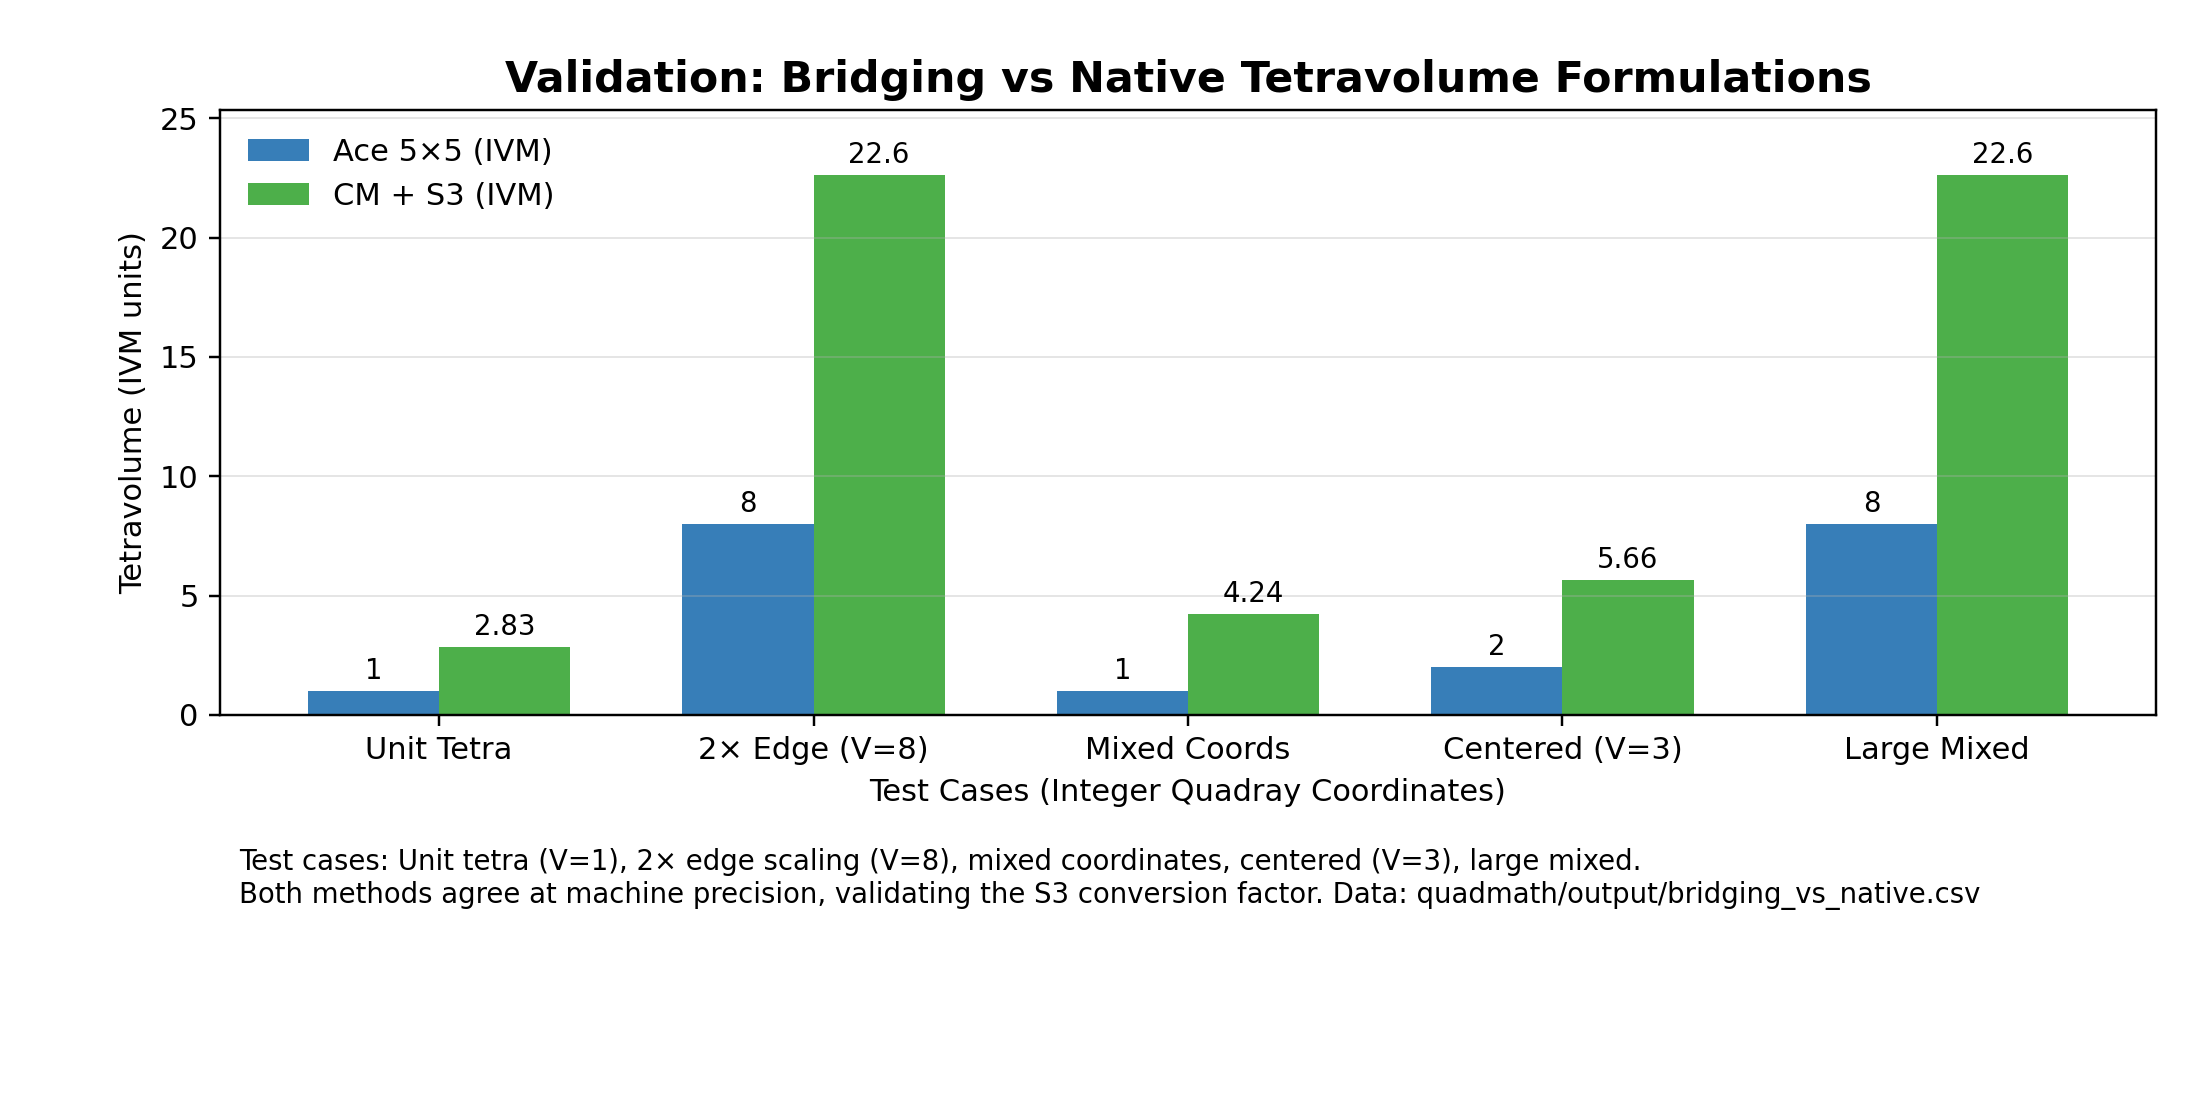
\includegraphics[width=0.9\textwidth]{figures/bridging_vs_native.png}
\caption{**Validation of bridging vs native tetravolume formulations across canonical examples**. This bar chart compares IVM tetravolumes computed via two independent methods: the "bridging" approach using Cayley–Menger determinants on Euclidean edge lengths converted to IVM units via the synergetics factor $S3=\sqrt{9/8}$, versus the "native" approach using Tom Ace's 5×5 determinant formula that operates directly on Quadray coordinates without XYZ intermediates. **Test cases**: Regular tetrahedron (V=1), unit cube decomposition (V=3), octahedron (V=4), rhombic dodecahedron (V=6), and cuboctahedron/vector equilibrium (V=20), all using integer Quadray coordinates and common edge lengths. **Results**: The overlapping bars demonstrate numerical agreement at machine precision between the length-based Coxeter.4D approach (Cayley–Menger + S3 conversion) and the coordinate-based Fuller.4D approach (Ace 5×5), confirming the mathematical equivalence of these formulations under synergetics unit conventions. Raw numerical data saved as \texttt{bridging\_vs\_native.csv} for reproducibility and further analysis.}
\label{fig:bridging_native}
\end{figure}

\begin{figure}[htbp]
\centering
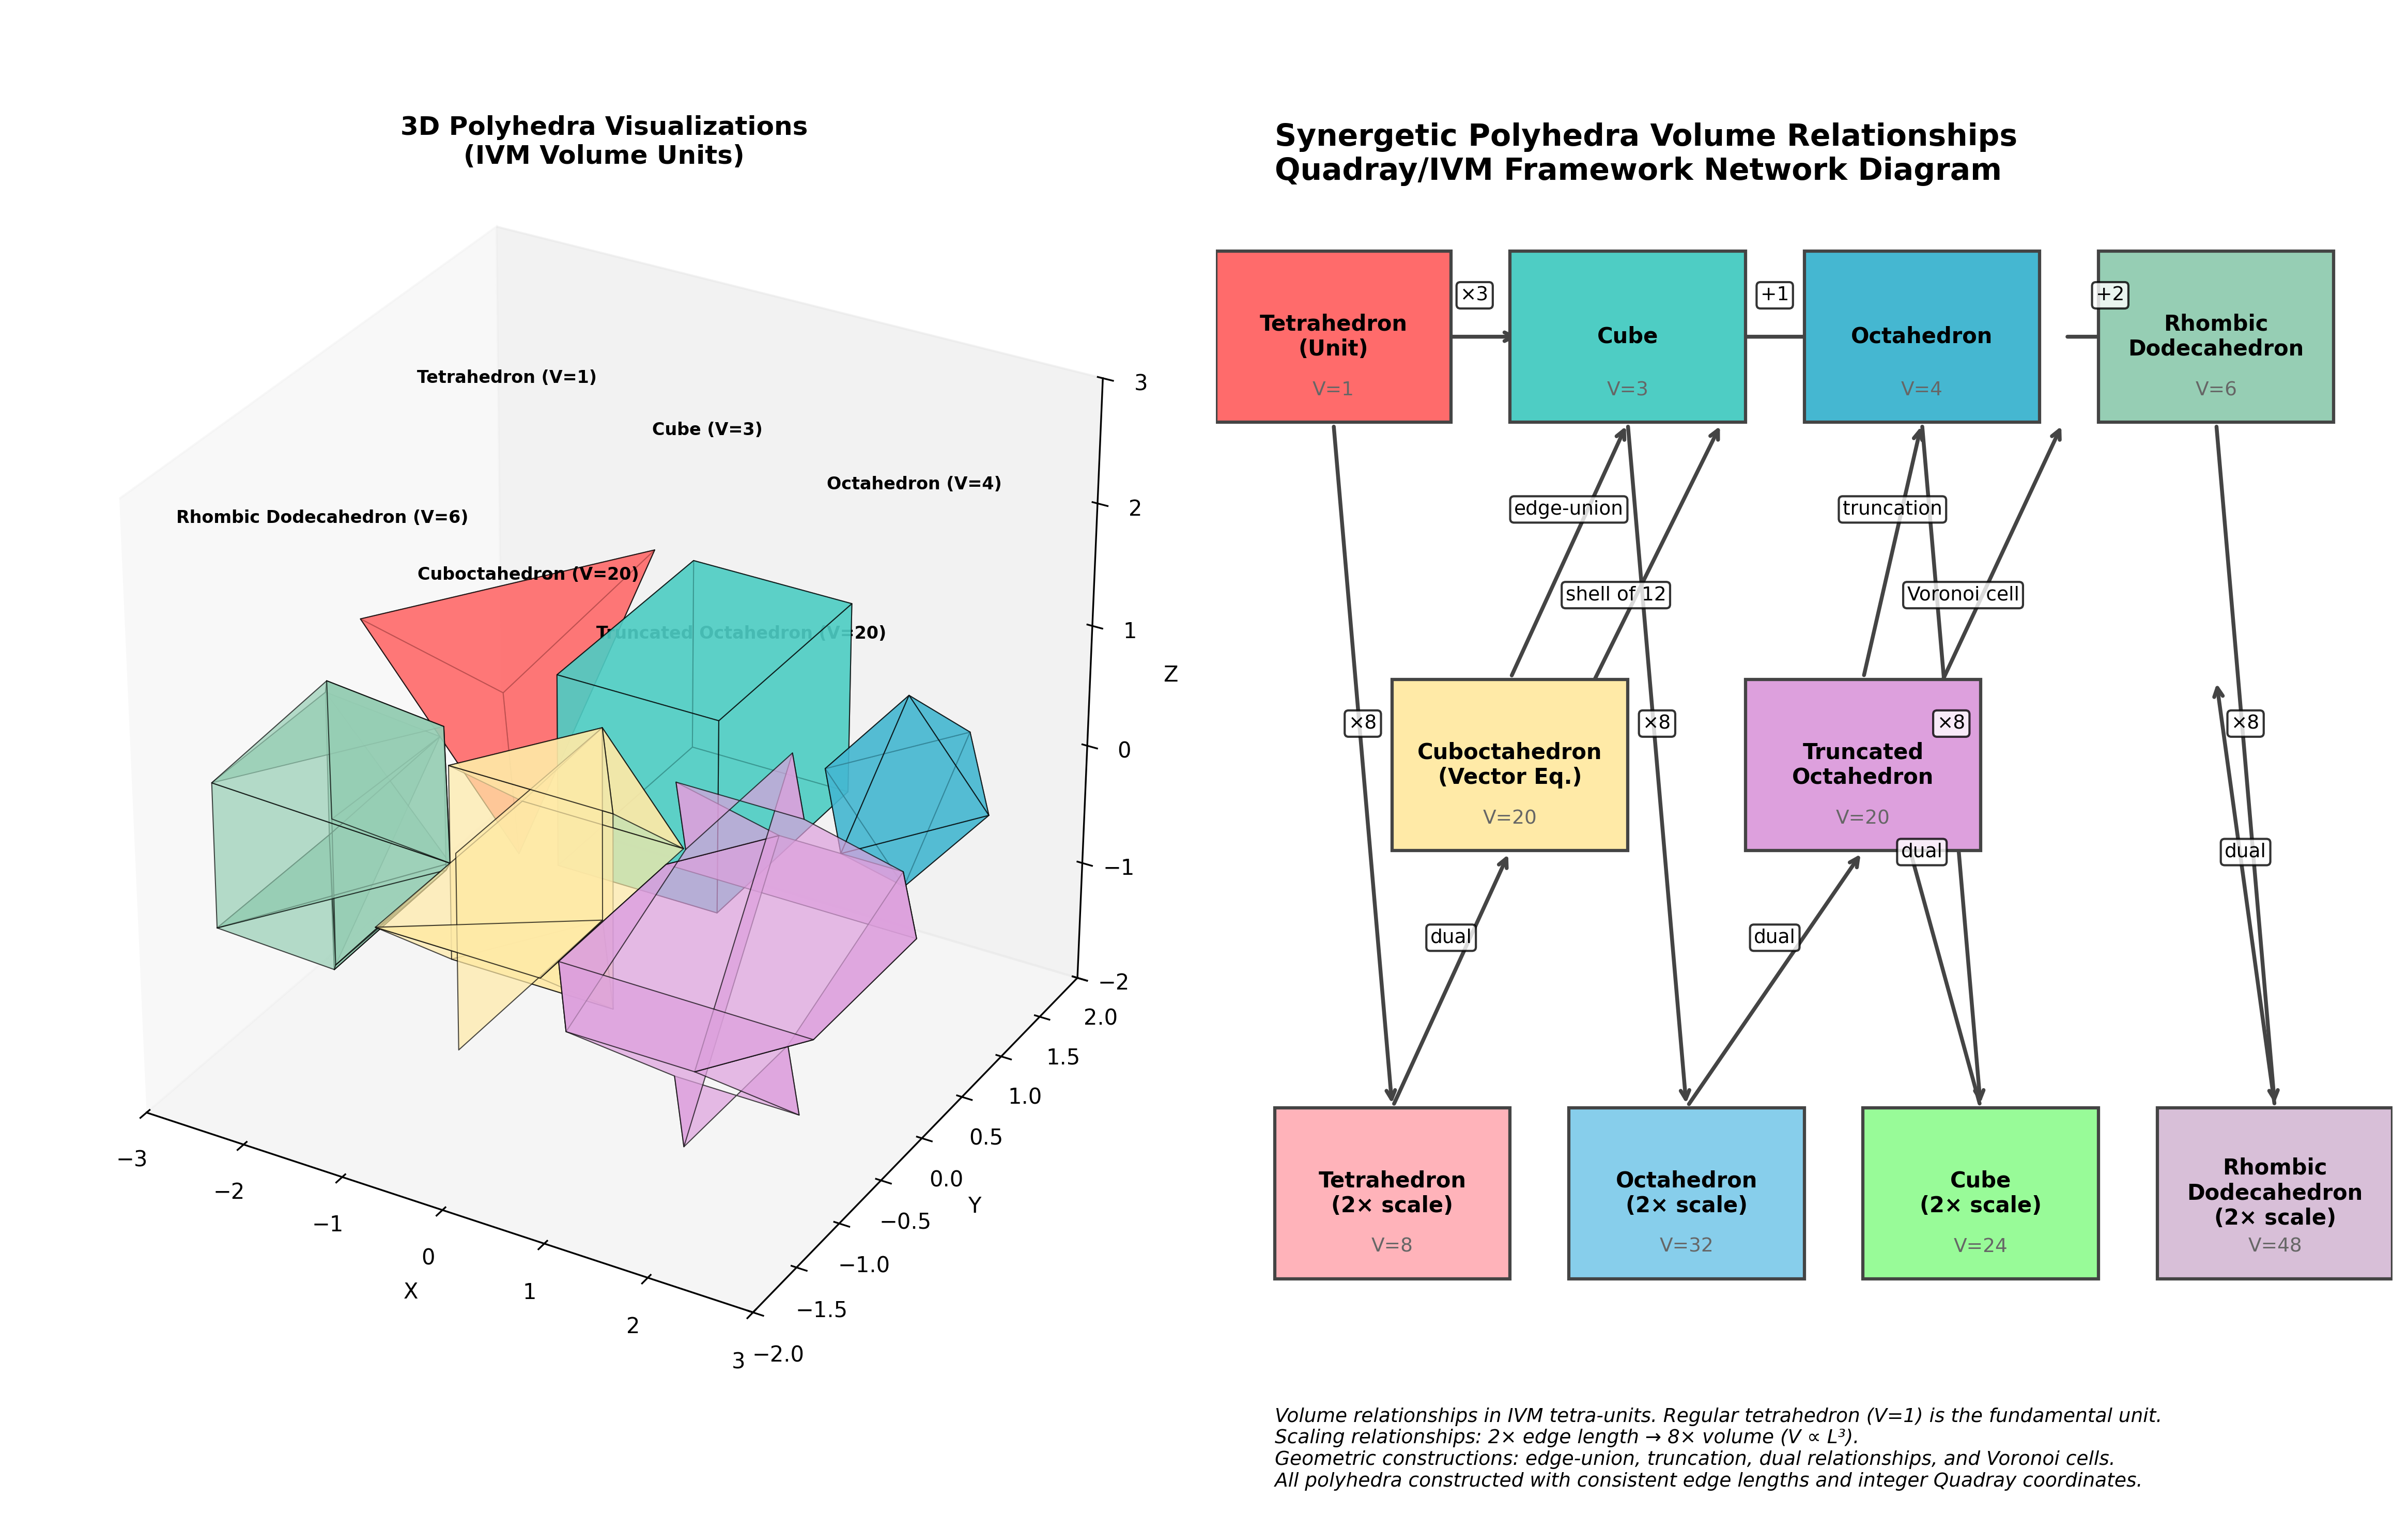
\includegraphics[width=0.9\textwidth]{figures/polyhedra_quadray_constructions.png}
\caption{**Synergetic polyhedra volume relationships in the Quadray/IVM framework (network diagram)**. This schematic illustrates the hierarchical volume relationships among key polyhedra when constructed with consistent edge lengths and expressed as integer-coordinate linear combinations of Quadray basis vectors. **Nodes (volumes in IVM tetra-units)**: Regular tetrahedron (V=1, fundamental unit), cube (V=3), octahedron (V=4), rhombic dodecahedron (V=6), and cuboctahedron/vector equilibrium (V=20). **Directed arrows (geometric relationships)**: The cube emerges as approximately 3× the tetrahedron volume through orthogonal space-filling; the octahedron (V=4) forms from edge-midpoint unions on the tetrahedral frame; the rhombic dodecahedron (V=6) serves as the Voronoi cell of the FCC/CCP lattice when centered at the origin; the cuboctahedron (V=20) represents the shell of twelve nearest IVM neighbors at permutations of $(2,1,1,0)$ Quadray coordinates. **Fuller.4D significance**: These integer volume ratios reflect the quantized nature of space-filling in synergetics, where the regular tetrahedron provides a natural unit container and other polyhedra emerge as integer multiples, supporting discrete geometric computation and exact lattice-based optimization methods. All constructions respect the IVM unit convention where the regular tetrahedron has tetravolume 1.}
\label{fig:polyhedra_quadray_map}
\end{figure}

\hypertarget{short-python-snippets-paper-reproducibility}{%
\subsubsection{Short Python snippets (paper
reproducibility)}\label{short-python-snippets-paper-reproducibility}}

\begin{Shaded}
\begin{Highlighting}[]
\ImportTok{from}\NormalTok{ quadray }\ImportTok{import}\NormalTok{ Quadray, ace\_tetravolume\_5x5}

\NormalTok{o }\OperatorTok{=}\NormalTok{ Quadray(}\DecValTok{0}\NormalTok{,}\DecValTok{0}\NormalTok{,}\DecValTok{0}\NormalTok{,}\DecValTok{0}\NormalTok{)}
\NormalTok{p }\OperatorTok{=}\NormalTok{ Quadray(}\DecValTok{2}\NormalTok{,}\DecValTok{1}\NormalTok{,}\DecValTok{0}\NormalTok{,}\DecValTok{1}\NormalTok{)}
\NormalTok{q }\OperatorTok{=}\NormalTok{ Quadray(}\DecValTok{2}\NormalTok{,}\DecValTok{1}\NormalTok{,}\DecValTok{1}\NormalTok{,}\DecValTok{0}\NormalTok{)}
\NormalTok{r }\OperatorTok{=}\NormalTok{ Quadray(}\DecValTok{2}\NormalTok{,}\DecValTok{0}\NormalTok{,}\DecValTok{1}\NormalTok{,}\DecValTok{1}\NormalTok{)}
\ControlFlowTok{assert}\NormalTok{ ace\_tetravolume\_5x5(o,p,q,r) }\OperatorTok{==} \DecValTok{1}  \CommentTok{\# unit IVM tetra}
\end{Highlighting}
\end{Shaded}

\begin{Shaded}
\begin{Highlighting}[]
\ImportTok{import}\NormalTok{ numpy }\ImportTok{as}\NormalTok{ np}
\ImportTok{from}\NormalTok{ cayley\_menger }\ImportTok{import}\NormalTok{ ivm\_tetra\_volume\_cayley\_menger}

\CommentTok{\# Example: regular tetrahedron with edge length 1 (XYZ units)}
\NormalTok{d2 }\OperatorTok{=}\NormalTok{ np.ones((}\DecValTok{4}\NormalTok{,}\DecValTok{4}\NormalTok{)) }\OperatorTok{{-}}\NormalTok{ np.eye(}\DecValTok{4}\NormalTok{)  }\CommentTok{\# squared distances}
\NormalTok{V\_ivm }\OperatorTok{=}\NormalTok{ ivm\_tetra\_volume\_cayley\_menger(d2)   }\CommentTok{\# = 1/8 in IVM tetra{-}units}
\end{Highlighting}
\end{Shaded}

\begin{Shaded}
\begin{Highlighting}[]
\CommentTok{\# SymPy implementation of Tom Ace 5×5 (symbolic determinant)}
\ImportTok{from}\NormalTok{ sympy }\ImportTok{import}\NormalTok{ Matrix}

\KeywordTok{def}\NormalTok{ qvolume(q0, q1, q2, q3):}
\NormalTok{    M }\OperatorTok{=}\NormalTok{ Matrix([}
\NormalTok{        q0 }\OperatorTok{+}\NormalTok{ (}\DecValTok{1}\NormalTok{,),}
\NormalTok{        q1 }\OperatorTok{+}\NormalTok{ (}\DecValTok{1}\NormalTok{,),}
\NormalTok{        q2 }\OperatorTok{+}\NormalTok{ (}\DecValTok{1}\NormalTok{,),}
\NormalTok{        q3 }\OperatorTok{+}\NormalTok{ (}\DecValTok{1}\NormalTok{,),}
\NormalTok{        [}\DecValTok{1}\NormalTok{, }\DecValTok{1}\NormalTok{, }\DecValTok{1}\NormalTok{, }\DecValTok{1}\NormalTok{, }\DecValTok{0}\NormalTok{],}
\NormalTok{    ])}
    \ControlFlowTok{return} \BuiltInTok{abs}\NormalTok{(M.det()) }\OperatorTok{/} \DecValTok{4}
\end{Highlighting}
\end{Shaded}

\begin{Shaded}
\begin{Highlighting}[]
\CommentTok{\# Symbolic variant with SymPy (exact radicals)}
\ImportTok{from}\NormalTok{ sympy }\ImportTok{import}\NormalTok{ Matrix, sqrt, simplify}
\ImportTok{from}\NormalTok{ symbolic }\ImportTok{import}\NormalTok{ cayley\_menger\_volume\_symbolic, convert\_xyz\_volume\_to\_ivm\_symbolic}

\NormalTok{d2 }\OperatorTok{=}\NormalTok{ Matrix([[}\DecValTok{0}\NormalTok{,}\DecValTok{1}\NormalTok{,}\DecValTok{1}\NormalTok{,}\DecValTok{1}\NormalTok{],[}\DecValTok{1}\NormalTok{,}\DecValTok{0}\NormalTok{,}\DecValTok{1}\NormalTok{,}\DecValTok{1}\NormalTok{],[}\DecValTok{1}\NormalTok{,}\DecValTok{1}\NormalTok{,}\DecValTok{0}\NormalTok{,}\DecValTok{1}\NormalTok{],[}\DecValTok{1}\NormalTok{,}\DecValTok{1}\NormalTok{,}\DecValTok{1}\NormalTok{,}\DecValTok{0}\NormalTok{]])}
\NormalTok{V\_xyz\_sym }\OperatorTok{=}\NormalTok{ cayley\_menger\_volume\_symbolic(d2)      }\CommentTok{\# sqrt(2)/12}
\NormalTok{V\_ivm\_sym }\OperatorTok{=}\NormalTok{ simplify(convert\_xyz\_volume\_to\_ivm\_symbolic(V\_xyz\_sym))  }\CommentTok{\# 1/8}
\end{Highlighting}
\end{Shaded}

\hypertarget{random-tetrahedra-in-the-ivm-integer-volumes}{%
\subsubsection{Random tetrahedra in the IVM (integer
volumes)}\label{random-tetrahedra-in-the-ivm-integer-volumes}}

\begin{itemize}
\tightlist
\item
  The 12 CCP directions are the permutations of \((2,1,1,0)\). Random
  walks on this move set generate integer-coordinate Quadrays; resulting
  tetrahedra have integer tetravolumes.
\end{itemize}

\begin{Shaded}
\begin{Highlighting}[]
\ImportTok{from}\NormalTok{ itertools }\ImportTok{import}\NormalTok{ permutations}
\ImportTok{from}\NormalTok{ random }\ImportTok{import}\NormalTok{ choice}
\ImportTok{from}\NormalTok{ quadray }\ImportTok{import}\NormalTok{ Quadray, ace\_tetravolume\_5x5}

\NormalTok{moves }\OperatorTok{=}\NormalTok{ [Quadray(}\OperatorTok{*}\NormalTok{p) }\ControlFlowTok{for}\NormalTok{ p }\KeywordTok{in} \BuiltInTok{set}\NormalTok{(permutations((}\DecValTok{2}\NormalTok{,}\DecValTok{1}\NormalTok{,}\DecValTok{1}\NormalTok{,}\DecValTok{0}\NormalTok{)))]}

\KeywordTok{def}\NormalTok{ random\_walk(start: Quadray, steps: }\BuiltInTok{int}\NormalTok{) }\OperatorTok{{-}\textgreater{}}\NormalTok{ Quadray:}
\NormalTok{    cur }\OperatorTok{=}\NormalTok{ start}
    \ControlFlowTok{for}\NormalTok{ \_ }\KeywordTok{in} \BuiltInTok{range}\NormalTok{(steps):}
\NormalTok{        m }\OperatorTok{=}\NormalTok{ choice(moves)}
\NormalTok{        cur }\OperatorTok{=}\NormalTok{ Quadray(cur.a}\OperatorTok{+}\NormalTok{m.a, cur.b}\OperatorTok{+}\NormalTok{m.b, cur.c}\OperatorTok{+}\NormalTok{m.c, cur.d}\OperatorTok{+}\NormalTok{m.d)}
    \ControlFlowTok{return}\NormalTok{ cur}

\NormalTok{A }\OperatorTok{=}\NormalTok{ random\_walk(Quadray(}\DecValTok{0}\NormalTok{,}\DecValTok{0}\NormalTok{,}\DecValTok{0}\NormalTok{,}\DecValTok{0}\NormalTok{), }\DecValTok{1000}\NormalTok{)}
\NormalTok{B }\OperatorTok{=}\NormalTok{ random\_walk(Quadray(}\DecValTok{0}\NormalTok{,}\DecValTok{0}\NormalTok{,}\DecValTok{0}\NormalTok{,}\DecValTok{0}\NormalTok{), }\DecValTok{1000}\NormalTok{)}
\NormalTok{C }\OperatorTok{=}\NormalTok{ random\_walk(Quadray(}\DecValTok{0}\NormalTok{,}\DecValTok{0}\NormalTok{,}\DecValTok{0}\NormalTok{,}\DecValTok{0}\NormalTok{), }\DecValTok{1000}\NormalTok{)}
\NormalTok{D }\OperatorTok{=}\NormalTok{ random\_walk(Quadray(}\DecValTok{0}\NormalTok{,}\DecValTok{0}\NormalTok{,}\DecValTok{0}\NormalTok{,}\DecValTok{0}\NormalTok{), }\DecValTok{1000}\NormalTok{)}
\NormalTok{V }\OperatorTok{=}\NormalTok{ ace\_tetravolume\_5x5(A,B,C,D)            }\CommentTok{\# integer}
\end{Highlighting}
\end{Shaded}

\hypertarget{algebraic-precision}{%
\subsubsection{Algebraic precision}\label{algebraic-precision}}

\begin{itemize}
\tightlist
\item
  Determinants via floating-point introduce rounding noise. For exact
  arithmetic, use the
  \href{https://en.wikipedia.org/wiki/Bareiss_algorithm}{Bareiss
  algorithm} (already used by \texttt{ace\_tetravolume\_5x5}) or
  symbolic engines (e.g., \texttt{sympy}). For large random-walk
  examples with integer inputs, volumes are exact integers.
\item
  When computing via XYZ determinants, high-precision floats (e.g.,
  \texttt{gmpy2.mpfr}) or symbolic matrices avoid vestigial errors;
  round at the end if the underlying result is known to be integral.
\end{itemize}

\hypertarget{xyz-determinant-and-the-s3-conversion}{%
\subsubsection{XYZ determinant and the S3
conversion}\label{xyz-determinant-and-the-s3-conversion}}

\begin{itemize}
\tightlist
\item
  Using XYZ coordinates of the four vertices: see Eq. \eqref{eq:xyz_det}
  for the determinant form and the S3 conversion to IVM units.
\end{itemize}

\hypertarget{d3-vs-r3-60-closing-the-lid-vs-orthogonal-cubing}{%
\subsubsection{D\^{}3 vs R\^{}3: 60° ``closing the lid'' vs orthogonal
``cubing''}\label{d3-vs-r3-60-closing-the-lid-vs-orthogonal-cubing}}

\begin{itemize}
\tightlist
\item
  \textbf{IVM (D\^{}3) heuristic}: From a 60--60--60 corner, three
  non-negative edge lengths \(A,B,C\) along quadray directions enclose a
  tetrahedron by ``closing the lid.'' In synergetics, the tetravolume
  scales as the simple product \(ABC\) under IVM conventions (unit
  regular tetra has volume 1). By contrast, in the orthogonal (R\^{}3)
  habit, one constructs a full parallelepiped (12 edges); the tetra
  occupies one-sixth of the triple product of edge vectors. The IVM path
  is more direct for tetrahedra.
\item
  \textbf{Pedagogical note}: Adopt a vector-first approach. Differences
  like \((P_i-P_0)\) denote edge vectors; Quadrays and Cartesian can be
  taught in parallel as vector languages on the same Euclidean
  container.
\end{itemize}

Reference notebook with worked examples and code:
\href{https://github.com/4dsolutions/School_of_Tomorrow/blob/master/Qvolume.ipynb}{Tetravolumes
with Quadrays (Qvolume.ipynb)}.

See implementation: \texttt{tetra\_volume\_cayley\_menger}.

\begin{itemize}
\tightlist
\item
  Lattice projection: round to nearest integer quadray; renormalize to
  maintain non-negativity and a minimal zero.
\end{itemize}

\hypertarget{code-methods-anchors}{%
\subsection{Code methods (anchors)}\label{code-methods-anchors}}

\hypertarget{code:integer_tetra_volume}{%
\subsubsection{\texorpdfstring{\texttt{integer\_tetra\_volume}}{integer\_tetra\_volume}}\label{code:integer_tetra_volume}}

Source: \texttt{src/quadray.py} --- integer 3×3 determinant for lattice
tetravolume.

\hypertarget{code:ace_tetravolume_5x5}{%
\subsubsection{\texorpdfstring{\texttt{ace\_tetravolume\_5x5}}{ace\_tetravolume\_5x5}}\label{code:ace_tetravolume_5x5}}

Source: \texttt{src/quadray.py} --- Tom Ace 5×5 determinant in IVM
units.

\hypertarget{code:tetra_volume_cayley_menger}{%
\subsubsection{\texorpdfstring{\texttt{tetra\_volume\_cayley\_menger}}{tetra\_volume\_cayley\_menger}}\label{code:tetra_volume_cayley_menger}}

Source: \texttt{src/cayley\_menger.py} --- length-based formula (XYZ
units).

\hypertarget{code:ivm_tetra_volume_cayley_menger}{%
\subsubsection{\texorpdfstring{\texttt{ivm\_tetra\_volume\_cayley\_menger}}{ivm\_tetra\_volume\_cayley\_menger}}\label{code:ivm_tetra_volume_cayley_menger}}

Source: \texttt{src/cayley\_menger.py} --- Cayley--Menger volume
converted to IVM units.

\hypertarget{code:urner_embedding}{%
\subsubsection{\texorpdfstring{\texttt{urner\_embedding}}{urner\_embedding}}\label{code:urner_embedding}}

Source: \texttt{src/conversions.py} --- canonical XYZ embedding.

\hypertarget{code:quadray_to_xyz}{%
\subsubsection{\texorpdfstring{\texttt{quadray\_to\_xyz}}{quadray\_to\_xyz}}\label{code:quadray_to_xyz}}

Source: \texttt{src/conversions.py} --- apply embedding matrix to map
Quadray to XYZ.

\hypertarget{code:bareiss_determinant_int}{%
\subsubsection{\texorpdfstring{\texttt{bareiss\_determinant\_int}}{bareiss\_determinant\_int}}\label{code:bareiss_determinant_int}}

Source: \texttt{src/linalg\_utils.py} --- exact integer Bareiss
determinant.

\hypertarget{information-geometry-methods-anchors}{%
\subsubsection{Information geometry methods
(anchors)}\label{information-geometry-methods-anchors}}

\hypertarget{code:fisher_information_matrix}{%
\paragraph{\texorpdfstring{\texttt{fisher\_information\_matrix}}{fisher\_information\_matrix}}\label{code:fisher_information_matrix}}

Source: \texttt{src/information.py} --- empirical outer-product
estimator.

\hypertarget{code:natural_gradient_step}{%
\paragraph{\texorpdfstring{\texttt{natural\_gradient\_step}}{natural\_gradient\_step}}\label{code:natural_gradient_step}}

Source: \texttt{src/information.py} --- damped inverse-Fisher step.

\hypertarget{code:free_energy}{%
\paragraph{\texorpdfstring{\texttt{free\_energy}}{free\_energy}}\label{code:free_energy}}

Source: \texttt{src/information.py} --- discrete-state variational free
energy.

\hypertarget{code:discrete_ivm_descent}{%
\paragraph{\texorpdfstring{\texttt{discrete\_ivm\_descent}}{discrete\_ivm\_descent}}\label{code:discrete_ivm_descent}}

Source: \texttt{src/discrete\_variational.py} --- greedy integer-valued
descent over the IVM using canonical neighbor moves; returns a
\texttt{DiscretePath} with visited Quadrays and objective values. Pairs
with \texttt{animate\_discrete\_path}.

\hypertarget{code:animate_discrete_path}{%
\paragraph{\texorpdfstring{\texttt{animate\_discrete\_path}}{animate\_discrete\_path}}\label{code:animate_discrete_path}}

Source: \texttt{src/visualize.py} --- animate a \texttt{DiscretePath} to
MP4; saves CSV/NPZ trajectory to \texttt{quadmath/output/}.

Relevant tests (\texttt{tests/}):

\begin{itemize}
\tightlist
\item
  \texttt{test\_quadray.py} (unit IVM tetra, divisibility-by-4 scaling,
  Ace vs.~integer method)
\item
  \texttt{test\_quadray\_cov.py} (Ace determinant basic check)
\item
  \texttt{test\_cayley\_menger.py} (regular tetra volume in XYZ units)
\item
  \texttt{test\_linalg\_utils.py} (Bareiss determinant behavior)
\item
  \texttt{test\_examples.py}, \texttt{test\_examples\_cov.py}
  (neighbors, examples)
\item
  \texttt{test\_metrics.py}, \texttt{test\_metrics\_cov.py},
  \texttt{test\_information.py}, \texttt{test\_paths.py},
  \texttt{test\_paths\_cov.py}
\end{itemize}

\hypertarget{reproducibility-checklist}{%
\subsection{Reproducibility checklist}\label{reproducibility-checklist}}

\begin{itemize}
\tightlist
\item
  All formulas used in the paper are implemented in \texttt{src/} and
  verified by \texttt{tests/}.
\item
  Determinants are computed with exact arithmetic for integer inputs;
  floating-point paths are used only where appropriate and results are
  converted (e.g., via S3) as specified.
\item
  Random-walk experiments produce integer volumes; Ace 5×5 determinant
  agrees with length-based methods.
\item
  Volume tracking: monitor integer simplex volume to detect convergence
  plateaus.
\item
  Face/edge analyses: interpret sensitivity along edges; subspace
  searches across faces.
\end{itemize}

\hypertarget{dsolutions-ecosystem-comprehensive-implementation-catalog}{%
\subsection{4dsolutions ecosystem: comprehensive implementation
catalog}\label{dsolutions-ecosystem-comprehensive-implementation-catalog}}

\hypertarget{primary-python-implementations-math-for-wisdom---m4w}{%
\subsubsection{Primary Python implementations (Math for Wisdom -
m4w)}\label{primary-python-implementations-math-for-wisdom---m4w}}

\begin{itemize}
\tightlist
\item
  \textbf{Quadray vectors and conversions}:
  \href{https://github.com/4dsolutions/m4w/blob/main/qrays.py}{\texttt{qrays.py}}
  --- defines a \texttt{Qvector} class with normalization
  (\texttt{norm}, \texttt{norm0}), vector arithmetic, XYZ bridging,
  cross products, and SymPy symbolic support. Key features include:

  \begin{itemize}
  \tightlist
  \item
    Projective normalization with \texttt{(k,k,k,k)} subtraction
  \item
    Length calculation: \(\sqrt{\frac{1}{2}(a^2+b^2+c^2+d^2)}\) after
    \texttt{norm0}
  \item
    Cross product implementation with \(\sqrt{2}/4\) scaling factor
  \item
    Comprehensive XYZ conversion matrices and rotation support
  \end{itemize}
\item
  \textbf{Synergetic tetravolumes and modules}:
  \href{https://github.com/4dsolutions/m4w/blob/main/tetravolume.py}{\texttt{tetravolume.py}}
  --- implements multiple volume algorithms (PdF, CM, GdJ), dihedral
  calculations, and BEAST module system:

  \begin{itemize}
  \tightlist
  \item
    \texttt{Tetrahedron} class with six edge lengths and multiple volume
    methods
  \item
    BEAST subclasses: A, B (volume 1/24), E (icosahedral), S, T modules
  \item
    Volume scaling by synergetics constant \(\sqrt{9/8}\)
  \item
    Integration with \texttt{qrays.py} for \texttt{qvolume} computations
  \end{itemize}
\end{itemize}

\hypertarget{educational-framework-school_of_tomorrow}{%
\subsubsection{Educational framework
(School\_of\_Tomorrow)}\label{educational-framework-school_of_tomorrow}}

\begin{itemize}
\tightlist
\item
  \textbf{Interactive algorithms}:
  \href{https://github.com/4dsolutions/School_of_Tomorrow}{School\_of\_Tomorrow}
  repository with comprehensive notebook tutorials:

  \begin{itemize}
  \tightlist
  \item
    \href{https://github.com/4dsolutions/School_of_Tomorrow/blob/master/Qvolume.ipynb}{\texttt{Qvolume.ipynb}}:
    Tom Ace 5×5 determinant method with random-walk demonstrations
  \item
    \href{https://github.com/4dsolutions/School_of_Tomorrow/blob/master/VolumeTalk.ipynb}{\texttt{VolumeTalk.ipynb}}:
    Comparative analysis of bridging (CM+S3) vs native (Ace/GdJ)
    tetravolume formulas
  \item
    \href{https://github.com/4dsolutions/School_of_Tomorrow/blob/master/QuadCraft_Project.ipynb}{\texttt{QuadCraft\_Project.ipynb}}:
    1,255 lines of interactive CCP navigation and volume calculations
  \end{itemize}
\item
  \textbf{Visualization modules}: Core Python modules for 3D rendering
  and animation:

  \begin{itemize}
  \tightlist
  \item
    \href{https://github.com/4dsolutions/School_of_Tomorrow/blob/master/quadcraft.py}{\texttt{quadcraft.py}}:
    POV-Ray scene generation with 15 test functions, CCP demonstrations,
    BRYG coordinate mapping
  \item
    \href{https://github.com/4dsolutions/School_of_Tomorrow/blob/master/flextegrity.py}{\texttt{flextegrity.py}}:
    Polyhedron framework with 26 named coordinate points, concentric
    hierarchy, automatic scene generation
  \end{itemize}
\end{itemize}

\hypertarget{cross-language-validation-and-extensions}{%
\subsubsection{Cross-language validation and
extensions}\label{cross-language-validation-and-extensions}}

\begin{itemize}
\item
  \textbf{Rust implementation}:
  \href{https://github.com/4dsolutions/rusty_rays}{\texttt{rusty\_rays}}
  --- performance-oriented Rust port with complete vector operations for
  both Vivm (IVM) and Vxyz coordinate systems, providing independent
  algorithmic validation.
\item
  \textbf{Clojure functional approach}:
  \href{https://github.com/4dsolutions/synmods}{\texttt{synmods}} ---
  functional programming implementation with protocol-based design,
  including
  \href{https://github.com/4dsolutions/synmods/blob/master/qrays.clj}{\texttt{qrays.clj}}
  and 26-point coordinate system.
\item
  \textbf{VPython animations}:
  \href{https://github.com/4dsolutions/BookCovers}{\texttt{BookCovers}}
  --- real-time educational animations with
  \href{https://github.com/4dsolutions/BookCovers/blob/master/bookdemo.py}{\texttt{bookdemo.py}},
  interactive controls, and live tetravolume tracking.
\item
  \textbf{Dedicated pedagogy}:
  \href{https://github.com/4dsolutions/tetravolumes}{\texttt{tetravolumes}}
  repository with
  \href{https://raw.githubusercontent.com/4dsolutions/tetravolumes/refs/heads/master/Computing\%20Volumes.ipynb}{\texttt{Computing\ Volumes.ipynb}}
  and algorithm-focused materials.
\end{itemize}

\hypertarget{api-correspondence-and-validation}{%
\subsubsection{API correspondence and
validation}\label{api-correspondence-and-validation}}

\textbf{Mapping to this codebase}: The external implementations provide
extensive validation and pedagogical context for our \texttt{src/}
modules:

\begin{longtable}[]{@{}lll@{}}
\toprule
\begin{minipage}[b]{0.30\columnwidth}\raggedright
4dsolutions module\strut
\end{minipage} & \begin{minipage}[b]{0.35\columnwidth}\raggedright
This codebase (\texttt{src/})\strut
\end{minipage} & \begin{minipage}[b]{0.26\columnwidth}\raggedright
Correspondence\strut
\end{minipage}\tabularnewline
\midrule
\endhead
\begin{minipage}[t]{0.30\columnwidth}\raggedright
\texttt{qrays.py::Qvector}\strut
\end{minipage} & \begin{minipage}[t]{0.35\columnwidth}\raggedright
\texttt{quadray.py::Quadray}\strut
\end{minipage} & \begin{minipage}[t]{0.26\columnwidth}\raggedright
Vector operations, normalization, dot products\strut
\end{minipage}\tabularnewline
\begin{minipage}[t]{0.30\columnwidth}\raggedright
\texttt{tetravolume.py::ivm\_volume}\strut
\end{minipage} & \begin{minipage}[t]{0.35\columnwidth}\raggedright
\texttt{ace\_tetravolume\_5x5}\strut
\end{minipage} & \begin{minipage}[t]{0.26\columnwidth}\raggedright
Tom Ace 5×5 determinant method\strut
\end{minipage}\tabularnewline
\begin{minipage}[t]{0.30\columnwidth}\raggedright
\texttt{tetravolume.py} (PdF/CM)\strut
\end{minipage} & \begin{minipage}[t]{0.35\columnwidth}\raggedright
\texttt{cayley\_menger.py}\strut
\end{minipage} & \begin{minipage}[t]{0.26\columnwidth}\raggedright
Length-based volume formulas with S3 conversion\strut
\end{minipage}\tabularnewline
\begin{minipage}[t]{0.30\columnwidth}\raggedright
\texttt{qrays.py::quadray} (XYZ→IVM)\strut
\end{minipage} & \begin{minipage}[t]{0.35\columnwidth}\raggedright
\texttt{conversions.py::urner\_embedding}\strut
\end{minipage} & \begin{minipage}[t]{0.26\columnwidth}\raggedright
Coordinate system bridging\strut
\end{minipage}\tabularnewline
\begin{minipage}[t]{0.30\columnwidth}\raggedright
BEAST modules (A,B,E,S,T)\strut
\end{minipage} & \begin{minipage}[t]{0.35\columnwidth}\raggedright
\texttt{examples.py} volume constructions\strut
\end{minipage} & \begin{minipage}[t]{0.26\columnwidth}\raggedright
Synergetic polyhedron relationships\strut
\end{minipage}\tabularnewline
\bottomrule
\end{longtable}

\textbf{Cross-repository validation}: The multi-language implementations
(Rust, Clojure, POV-Ray, VPython) serve as independent checks on
algorithmic correctness and provide performance comparisons across
computational paradigms. Educational notebooks demonstrate consistent
results across bridging (CM+S3) and native (Ace/GdJ) tetravolume
formulations.

\end{document}
